\chapter{Preliminaries}
\label{sec:prelims}

\begin{figure}
\begin{tabular}{@{}c@{}c@{}}
\begin{subfigure}[b]{0.55\textwidth}
\begin{center}
\begin{allLangEnvFoot}
~{\scriptsize \textcolor{mygray}{A0:}}~ type Str = SInvalid | SNil
~{\scriptsize \textcolor{mygray}{A1:}}~          | SCons (ch:i8, tail:Str).
~{\scriptsize \textcolor{mygray}{A2:}}~
~{\scriptsize \textcolor{mygray}{A3:}}~ fn is_empty (s : Str) : bool =
~{\scriptsize \textcolor{mygray}{A4:}}~    assuming $\neg$(s is SInvalid) do
~{\scriptsize \textcolor{mygray}{A5:}}~      s is SNil.
\end{allLangEnvFoot}
\end{center}
\caption{\label{fig:isemptyspec}Spec program}
\end{subfigure}%
&
\begin{subfigure}[b]{0.45\textwidth}
\begin{center}
\begin{allLangEnvFoot}
~{\scriptsize \textcolor{mygray}{B0:}}~ #include <stdbool.h>
~{\scriptsize \textcolor{mygray}{B1:}}~
~{\scriptsize \textcolor{mygray}{B2:}}~ bool is_empty(char* s) {
~{\scriptsize \textcolor{mygray}{B3:}}~   if (!s) return false;
~{\scriptsize \textcolor{mygray}{B4:}}~   return *s == 0;
~{\scriptsize \textcolor{mygray}{B5:}}~ }
\end{allLangEnvFoot}
\end{center}
\caption{\label{fig:isemptyc}C program}
\end{subfigure}%
\\
\begin{subfigure}[b]{0.55\textwidth}
\begin{center}
\begin{allLangEnvFoot}
~{\scriptsize \textcolor{mygray}{S0:}}~ bool is_empty(Str s) {
~{\scriptsize \textcolor{mygray}{S1:}}~   assume $\neg$(s is Sinvalid);
~{\scriptsize \textcolor{mygray}{S2:}}~   return s is SNil;
~{\scriptsize \textcolor{mygray}{SE:}}~ }
\end{allLangEnvFoot}
\end{center}
\caption{\label{fig:isemptyspecir}(Abstracted) Spec IR}
\end{subfigure}%
&
\begin{subfigure}[b]{0.45\textwidth}
\begin{center}
\begin{allLangEnvFoot}
~{\scriptsize \textcolor{mygray}{C0: }}~ bool is_empty(i32 s) {
~{\scriptsize \textcolor{mygray}{C1: }}~   if $(s = 0_{i32})$: return false;
~{\scriptsize \textcolor{mygray}{C2: }}~   return $\memRead{\mem{}}{0_{i32}}{i8}$ = $0_{i8}$;
~{\scriptsize \textcolor{mygray}{CE: }}~ }
\end{allLangEnvFoot}
\end{center}
\caption{\label{fig:isemptycir}(Abstracted) C IR}
\end{subfigure}%
\\
\end{tabular}
\caption{\label{fig:isemptyspecandcandirs}\SpecL{} and C programs along with their corresponding IRs for the {\tt is\_empty} procedure.}
\end{figure}


\section{The Specification Language : \SpecL{}}
\label{sec:speclang}
We start with an introduction to our specification language, called \SpecL{}.
\SpecL{} supports recursive algebraic data types (ADT) \cite{algebraicdatatypes} similar to the
ones available in functional languages such as Haskell \cite{marlow2010haskell} and SML \cite{standardmlspec}.
\SpecL{} does not support universal types but does allow ADTs which are mutually recursive.
Additionally, \SpecL{} is equipped with the following {\em scalar} types: \type{unit}, \type{bool} (boolean) and \type{i<N>} (fixed-width bitvectors).
ADTs can be thought of as `sum of product' types where each {\em data constructor} represents a variant (of the sum-type)
and the arguments to each data constructor represents its {\em fields} (of the product-type).
For example, the \type{List} type (defined at \apc{0} in \cref{fig:llAllocSpec}) has two variants \cons{LNil} and \cons{LCons}.
\cons{LNil} has no fields while \cons{LCons} has two fields \field{val} and \field{tail} of types \type{i32} and \type{List} respectively.
Additionally, \SpecL{} follows {\em equirecursive} typing rules i.e.
a \type{List} value $l$ and $\cons{LCons}(1_\type{i32}, l)$ have {\em equal} types.
Later in \cref{sec:valuegraph}, we further expand on ADTs in the context of a
graphical representation of values used as part of our proof discharge algorithm.
The language also borrows its expression grammar heavily from functional languages.
This includes {\tt let-in}, {\tt if-then-else}, {\tt match} and function application.
Pattern matching (i.e. deconstruction) of ADT values is achieved through {\tt match}.
Unlike functional languages, \SpecL{} only supports first order functions.
Also, \SpecL{} does not support partial function application.
Hence, we limit our attention to C programs containing only first order functions.
\SpecL{} is equipped with a special {\tt assuming-do} construct for explicitly providing assertions.
\Cref{fig:isemptyspec} shows a \SpecL{} program with the {\tt assuming-do} construct, with its C equivalent
shown in \cref{fig:isemptyc}.
The corresponding IRs are shown in \cref{fig:isemptyspecir,fig:isemptycir} respectively.
The significance of explicit assertions in \SpecL{} is further discussed throughout this chapter.
\SpecL{} also provides intrinsic scalar operators for expressing computation in C succintly yet explicitly.
Examples of scalar operators include (a) logical operators (e.g., {\tt and}), (b) bitvector arithmatic operators (e.g., {\tt bvadd(+)}),
and (c) relational operators for comparing bitvectors interpreted as unsigned or signed integers (e.g., {\tt $\leq_{\tt u,s}$}).
The equality operator ($=$) is only supported for scalar types.

\begin{figure}[H]
\begin{small}
\begin{tabular}{rcl}
\nonTerm{expr} & $\rightarrow$ & \term{if} \nonTerm{expr} \term{then} \nonTerm{expr} \term{else} \nonTerm{expr} \\
& $|$ & \term{let} \nonTerm{id} \term{=} \nonTerm{expr} \term{in} \nonTerm{expr} \\
& $|$ & \term{match} \nonTerm{expr} \term{with} \nonTerm{match-clause-list} \\
& $|$ & \term{assuming} \nonTerm{expr} \term{do} \nonTerm{expr} \\
& $|$ & \nonTerm{id} \term{(} \nonTerm{expr-list} \term{)} \\
& $|$ & \nonTerm{data-cons} \term{(} \nonTerm{expr-list} \term{)} \\
& $|$ & \nonTerm{expr} \term{is} \nonTerm{data-cons} \\
& $|$ & \nonTerm{expr} \nonTerm{scalar-op} \nonTerm{expr} \\
& $|$ & \nonTerm{literal$_{\mathrm{Unit}}$} $|$ \nonTerm{literal$_{\mathrm{Bool}}$} $|$ \nonTerm{literal$_{\mathrm{i<N>}}$} \\
\\
\nonTerm{match-clause-list} & $\rightarrow$ & \nonTerm{match-clause}$^*$ \\
\nonTerm{match-clause} & $\rightarrow$ & \term{$|$} \nonTerm{data-cons} \term{(} \nonTerm{id-list} \term{)} \term{$\Rightarrow$} \nonTerm{expr} \\
\nonTerm{expr-list} & $\rightarrow$ & \term{$\epsilon$} \term{$|$} \nonTerm{expr} \term{,} \nonTerm{expr-list} \\
\nonTerm{id-list} & $\rightarrow$ & \term{$\epsilon$} \term{$|$} \nonTerm{id} \term{,} \nonTerm{id-list} \\
\\
\nonTerm{literal$_{\mathrm{Unit}}$} & $\rightarrow$ & \term{()} \\
\nonTerm{literal$_{\mathrm{Bool}}$} & $\rightarrow$ & \term{false} $|$ \term{true} \\
\nonTerm{literal$_{\mathrm{i<N>}}$} & $\rightarrow$ & [\term{0$\dots$2$^{\mathrm{N}}$-1}] \\
\end{tabular}
\end{small}
\caption{\label{fig:specgrammar}Simplified expression grammar of \SpecL{} language}
\end{figure}

\Cref{fig:specgrammar} shows the simplified expression grammar for \SpecL{} language.
\nonTerm{data-cons} represents an ADT data constructor.
The `\nonTerm{expr} {\tt is} \nonTerm{data-cons}' construct returns a value of \type{bool} type and is used to test whether
the value \nonTerm{expr} is of kind \nonTerm{data-cons}.
\nonTerm{scalar-op} includes the logical, arithmatic and relational operators supported by \SpecL{}.

\begin{figure}[t!]
\begin{tabular}{@{}c@{}c@{}}
\begin{subfigure}[b]{0.63\textwidth}
\begin{center}
\begin{allLangEnvFoot}
~{\scriptsize \textcolor{mygray}{A0:}}~ type List = LNil | LCons (val:i32, tail:List).
~{\scriptsize \textcolor{mygray}{A1:}}~
~{\scriptsize \textcolor{mygray}{A2:}}~ fn sum_list_impl (l:List) (sum:i32) :i32 =
~{\scriptsize \textcolor{mygray}{A3:}}~    match l with
~{\scriptsize \textcolor{mygray}{A4:}}~    | LNil => sum
~{\scriptsize \textcolor{mygray}{A5:}}~    | LCons(x, rest) =>
~{\scriptsize \textcolor{mygray}{A6:}}~                sum_list_impl(rest, sum + x).
~{\scriptsize \textcolor{mygray}{A7:}}~
~{\scriptsize \textcolor{mygray}{A8:}}~ fn sum_list (l:List) : i32 =
~{\scriptsize \textcolor{mygray}{A9:}}~    sum_list_impl(l, ${\tt 0_{i32}}$).
\end{allLangEnvFoot}
\end{center}
\caption{\label{fig:llTraverseSpec}Spec program}
\end{subfigure}%
&
\begin{subfigure}[b]{0.37\textwidth}
\begin{center}
\begin{allLangEnvFoot}
~{\scriptsize \textcolor{mygray}{S0:}}~ i32 sum_list (List l) {
~{\scriptsize \textcolor{mygray}{S1:}}~   i32 sum $\coloneqq$ ${\tt 0_{i32}}$;
~{\scriptsize \textcolor{mygray}{S2:}}~   while $\neg$(l is LNil):
~{\scriptsize \textcolor{mygray}{S3:}}~     // (l is LCons);
~{\scriptsize \textcolor{mygray}{S4:}}~     sum $\coloneqq$ sum + l.val;
~{\scriptsize \textcolor{mygray}{S5:}}~     l   $\coloneqq$ l.next;
~{\scriptsize \textcolor{mygray}{S6:}}~   return sum;
~{\scriptsize \textcolor{mygray}{SE:}}~ }
~{\scriptsize \textcolor{mygray}{}}~
~{\scriptsize \textcolor{mygray}{}}~
\end{allLangEnvFoot}
\end{center}
\caption{\label{fig:llTraverseSpecIR}(Abstracted) Spec IR}
\end{subfigure}%
\\
\begin{subfigure}[b]{0.63\textwidth}
\begin{center}
\begin{allLangEnvFoot}
~{\scriptsize \textcolor{mygray}{B0: }}~ typedef struct lnode {
~{\scriptsize \textcolor{mygray}{B1: }}~   unsigned val; struct lnode* next; } lnode;
~{\scriptsize \textcolor{mygray}{B2: }}~ 
~{\scriptsize \textcolor{mygray}{B3: }}~ unsigned sum_list(lnode* l) {
~{\scriptsize \textcolor{mygray}{B4: }}~   unsigned sum = 0;
~{\scriptsize \textcolor{mygray}{B5: }}~   while (l) {
~{\scriptsize \textcolor{mygray}{B6: }}~     sum += l$\rightarrow$val;
~{\scriptsize \textcolor{mygray}{B7: }}~     l = l$\rightarrow$next;
~{\scriptsize \textcolor{mygray}{B8: }}~   }
~{\scriptsize \textcolor{mygray}{B9: }}~   return sum;
~{\scriptsize \textcolor{mygray}{B10:}}~ }
\end{allLangEnvFoot}
\end{center}
\caption{\label{fig:llTraverseC}C program}
\end{subfigure}%
&
\begin{subfigure}[b]{0.37\textwidth}
\begin{center}
\begin{allLangEnvFoot}
~{\scriptsize \textcolor{mygray}{C0:}}~ i32 sum_list (i32 l) {
~{\scriptsize \textcolor{mygray}{C1:}}~   i32 sum $\coloneqq$ ${\tt 0_{i32}}$;
~{\scriptsize \textcolor{mygray}{C2:}}~   while ${\tt l \neq 0_{i32}}$:
~{\scriptsize \textcolor{mygray}{C3:}}~     sum $\coloneqq$ sum + $\structPointer{\tt l}{\mem{}}{lnode}{val}$;
~{\scriptsize \textcolor{mygray}{C4:}}~     l   $\coloneqq$ $\structPointer{\tt l}{\mem{}}{lnode}{next}$;
~{\scriptsize \textcolor{mygray}{C5:}}~   return sum;
~{\scriptsize \textcolor{mygray}{CE:}}~ }
~{\scriptsize \textcolor{mygray}{}}~
~{\scriptsize \textcolor{mygray}{}}~
~{\scriptsize \textcolor{mygray}{}}~
\end{allLangEnvFoot}
\vspace{7px}
\end{center}
\caption{\label{fig:llTraverseCIR}(Abstracted) C IR}
\end{subfigure}%
\\
\end{tabular}
\caption{\label{fig:llTraverseSpecAndCAndIRs}\SpecL{} and C programs for traversing a Linked List along with corresponding IRs for the {\tt sum\_list} procedures.}
\end{figure}


\section{Abstract Representation of Programs}
\label{sec:ir}
As outlined in \cref{sec:motivatingexample}, we convert both \SpecL{} and C programs to a common
abstract representation called the {\em Control Flow Graph} (CFG for short).
This process involves converting both programs to a linear representation called the IR.
This section presents both IR and CFG representations for the original \SpecL{} and C programs.

\subsection{Conversion of Programs to Intermediate Representation}
\label{sec:irconv}
IR is a Three-Address-Code (3AC) style intermediate representation.
We often omit intermediate registers in the IR for brevity, and refer to this as the {\em abstracted} IR.
We have already seen the IRs (in \cref{fig:llAllocSpecIR,fig:llAllocCIR}) for the \SpecL{} and C programs
that construct lists in \cref{fig:llAllocSpec,fig:llAllocC}.
\Cref{fig:llTraverseSpec,fig:llTraverseC} show \SpecL{} and C programs that traverse a list of integers
and compute their sum.
The corresponding IR programs for the above are shown in \cref{fig:llTraverseSpecIR,fig:llTraverseCIR} respectively.

The following major steps are performed during conversion of a \SpecL{} source to its IR representation:

\begin{enumerate}
\item {\tt match} statements are converted to explicit {\tt if-else} conditionals where each branch is
associated with a {\tt match} branch. The {\em sum-is} operator is used in the condition to query
the top-level data constructor of an expression. The fields of the data constructor are bound to
variables using the {\em product-access} or {\em accessor} operator.
For example, the {\tt match} statement in \apc{3} (in \cref{fig:llTraverseSpec}) is lowered to {\tt if-else}
in \cref{fig:llTraverseSpecIR}, where `\sumIs{\comv{l}}{LCons}' is used to test whether \comv{l} is
of kind \cons{LCons} and `\prodAccess{\comv{l}}{val}' is used to extract the \field{val} field of \cons{LCons} data constructor.
Importantly, the expression `\prodAccess{e}{fi}' is well-formed iff `\sumIs{e}{\mathnormal{V}_{fi}}', where $V_\field{fi}$ represents the
data constructor containing the field \field{fi}.
The construction of the IR guarantees the well-formedness of all expressions.
\item All tail-recursive calls are converted to loops in the IR. However, all non-tail procedure calls are preserved as is.
This transformation enables direct correlation (during equivalence checking) of tail-calls in \SpecL{} with native loops in C.
For example, the tail recursive function {\tt sum\_list\_impl} in \apc{2} (in \cref{fig:llTraverseSpec}) is converted to a non-recursive function with a loop.
\item All {\em helper} functions\footnote{We use a special marker to designate a function as `helper' in \SpecL{}.
For simplicity, this marker is omitted and instead helper function names are ended with the `{\tt \_impl}' suffix.}
are inlined at their call-site.
We are only interested in proving equivalence of non-helper functions in \SpecL{} with their C counterparts.
For example, the helper function {\tt sum\_list\_impl} (now non-recursive due to previous step), is inlined
at call-site \apc{7} in \cref{fig:llTraverseSpec}.
\item {\tt assuming-do} statements are converted to their equivalent {\tt assume} instruction in the IR.
A \SpecL{} program is {\em well-defined} iff it satisfies all {\tt assume} clauses encountered during its execution.
These conditions are called {\em undefined behaviour assumes} or UB {\em assumes} for short.
For example, the {\tt assuming-do} statement in \apc{4} in \cref{fig:isemptyspec} is converted to an {\tt assume}
instruction in \spc{1} in \cref{fig:isemptyspecir}.
\end{enumerate}

Similarly, the following transformations are carried out during conversion of a C source to its IR:

\begin{enumerate}
\item Non-determinism in the original C program is determinized in the IR.
This includes concretizing the size and memory layouts of both scalar (e.g. \type{int})
and compound (e.g., \type{struct}) types, along with fixing the order of evaluation in case
it is unspecified.
For example, during conversion of C program in \cref{fig:llAllocC} to IR (in \cref{fig:llAllocCIR}),
the sizes of pointer and \type{unsigned} types are fixed to 32 bits (i.e. \type{i32}).
Similarly, the memory layout (including alignment and offset) of \type{lnode} struct defined in \bpc{0} (in \cref{fig:llAllocC}) is chosen.
The implications of determinizing the C program behaviour are further discussed in \cref{sec:spectocalgo}.
For now, it is sufficient to note that we are interested in equivalence between \SpecL{} and this determinized version of C.
\item The memory state of the C program is made explicit, represented using the byte-addressable array `\mem{}'.
Memory loads and stores are represented using explicit operations on \mem{}, e.g.,
(a) memory load in \cpc{3} in \cpc{4} in \cref{fig:llTraverseCIR}, and
(b) memory stores in \cpc{5} and \cpc{6} in \cref{fig:llAllocCIR}.
The memory load and store operators are defined promptly in \cref{sec:irops}
\item We annotate calls to memory allocation functions (e.g., {\tt malloc}) with their call-site, i.e., IR PC.
For example, {\tt malloc$_\cpc{4}$} is annotated with its call-site \cpc{4} in \cref{fig:llAllocCIR}.
These annotations are used by a points-to analysis done as part of our equivalence checking procedure,
and defined subsequently in \cref{sec:pointsToFormal}.
\end{enumerate}

\subsection{IR Instructions}
\label{sec:irops}
Note that both \SpecL{} and C programs are converted to the common IR.
On the \SpecL{} side, IR supports scalar as well as ADT types defined in the \SpecL{} program under consideration.
The IR also inherits the scalar operators available as part of \SpecL{}.
Each ADT value can be thought of as a key-value dictionary that maps each of its field names
to their respective values.
These key-value pairs are accessed using the previously introduced {\em accessor} operator,
e.g., \prodAccess{l}{val} and \prodAccess{l}{next} represents the first and second fields of the
\cons{LCons} data constructor in \cref{fig:llTraverseSpecIR}.
Recall that, the IR also allows querying the top-level variant of an ADT value using the
{\em sum-is} operator, e.g., \sumIs{l}{LNil} in \cref{fig:llTraverseSpecIR}.
The \field{val} field is associated with the \cons{LCons} data constructor and
evidently, \prodAccess{l}{val} (and \prodAccess{l}{next}) is only {\em well-formed} under \sumIs{l}{LCons}.
As discussed, the well-formedness of all {\em accessor} expressions are preserved during
construction of IR for a \SpecL{} program.
Using {\em accessor} and {\em sum-is} operators, a \type{List} value $l$ can be expanded as:

\begin{equation}
\label{eqn:specDeconstruct}
U_S: l = \sumIf{\sumIs{l}{LNil}} \  \sumThen{\cons{LNil}} \  \sumElse{\cons{LCons}(\prodAccess{l}{val}, \prodAccess{l}{next})}
\end{equation}

In this expanded representation of $l$,
the {\em sum-deconstruction} operator `\sumDtor{}'
conditionally deconstructs the sum type into its variants \cons{LNil} and \cons{LCons}.
The {\em underlined} \sumDtor{} operator is a stricter version of {\tt if-then-else}, and is only used for ADT values.
An \sumDtor{} expression $e$ (for an ADT type $T$) must satisfy the following properties:
(a) $e$ has exactly one branch for each data construction of $T$ (in the order they are defined),
and (b) the branch associated with the data constructor $V$ has the form $V(e_1,e_2,\dots)$ i.e. its top-level operator is $V$.
For example, an \sumDtor{} expression for the \type{List} type must be of the form:
`\sumIf{e_1} \sumThen{\cons{LNil}} \sumElse{\cons{LCons}(e_2,e_3)}' for some expressions $e_1,e_2,e_3$.
\Cref{eqn:specDeconstruct} is called the {\em unrolling procedure} for the \type{List} variable $l$.
We can similarly define the unrolling procedure for any ADT variable (based on the definition of the ADT).

On the C side, the size of a pointer is fixed\footnote{We choose an address width of 4 bytes or 32 bits throughout this thesis.}
and the memory state is modeled as a byte-addressable array over bitvectors (represented by \mem{}).
``\memRead{\mem{}}{p}{T}'' represents a memory load operation and is equal to the bytes
at addresses [$p$, $p$+\sizeof{T}) in \mem{}, interpreted as a value of type \type{T}.
Similarly, ``\memWrite{\mem{}}{p}{v}{T}'' represents a memory store operation and is equal to \mem{}
everywhere except at addresses [$p$, $p$+\sizeof{T}) which contains
the value $v$ of type \type{T} (e.g., \cpc{5} in \cref{fig:llAllocCIR}).
We use the following two C-like syntaxes to represent more intricate memory loads succintly:

\begin{enumerate}
\item ``\structPointer{p}{\mem{}}{T}{fi}'' is equivalent to ``\memRead{\mem}{p+\offsetof{T}{fi}}{\typeof{T.fi}}''
i.e., it returns the bytes in the memory array \mem{} starting at address `$p+\offsetof{T}{fi}$'
and interpreted as a value of type \typeof{T.fi}.

\item ``\arrIndex{p}{i}{\mem{}}{T}'' is equivalent to ``\memRead{\mem}{p+i \times \sizeof{T}}{T}''
i.e., it returns the bytes in the memory array \mem{} starting at address `$p+i \times \sizeof{T}$'
and interpreted as a value of type \type{T}.
Interestingly, $\memRead{\mem{}}{p}{T} = \arrIndex{p}{0}{\mem{}}{}$.
\end{enumerate}

Recall that the size and layout of each type in C is concretized in the IR,
and hence the values `\offsetof{T}{f}' and `\sizeof{T}' are constants.
We use the `\addrof{}' operator to extract the address of a memory load expression:
``\addrof{\memRead{\mem{}}{p}{T}}'' is equivalent to $p$.
For example, at PC \cpc{5} in \cref{fig:llAllocCIR}, $\addrof{\structPointer{\mathnormal{p}}{\mem{}}{lnode}{val}} \Leftrightarrow p+\offsetof{lnode}{val}$.
Additionally, given a bitvector expression $e$, ``$e{\tt [ub:lb]}$'' represents a bitvector extract operation that extracts the bits
in the range [lb,ub] from $e$ resulting in a $(ub-lb+1)$-sized bitvector expression.

\begin{figure}[t!]
\begin{tabular}{@{}c@{}c@{}}
\begin{subfigure}[b]{0.5\textwidth}
\begin{center}
{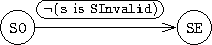
\includegraphics[scale=1.4]{chapters/figures/figIsEmptySpecCFG.pdf}}
\end{center}
\vspace{20px}
\caption{\label{fig:isemptyspeccfg}CFG of \SpecL{} procedure}
\end{subfigure}%
&
\begin{subfigure}[b]{0.5\textwidth}
\begin{center}
{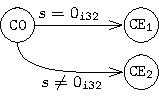
\includegraphics[scale=1.4]{chapters/figures/figIsEmptyCCFG.pdf}}
\end{center}
\caption{\label{fig:isemptyccfg}CFG of C procedure}
\end{subfigure}%
\\
\end{tabular}
\caption{\label{fig:isemptyspecandccfg}CFG representation of \SpecL{} and C IRs in \cref{fig:isemptyspecir,fig:isemptycir} for the {\tt is\_empty} procedures in \cref{fig:isemptyspec,fig:isemptyc} respectively.}
% \end{figure}

\begin{figure}
\begin{tabular}{@{}c@{}c@{}}
\begin{subfigure}[b]{0.5\textwidth}
\begin{center}
{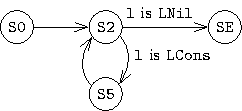
\includegraphics[scale=1.4]{chapters/figures/figSumListSpecCfg.pdf}}
\end{center}
\caption{\label{fig:llTraverseSpecCFG}CFG of \SpecL{} program}
\end{subfigure}%
&
\begin{subfigure}[b]{0.5\textwidth}
\begin{center}
{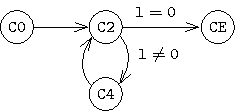
\includegraphics[scale=1.4]{chapters/figures/figSumListCCfg.pdf}}
\end{center}
\caption{\label{fig:llTraverseCCFG}CFG of C program}
\end{subfigure}%
\\
\end{tabular}
\caption{\label{fig:llTraverseSpecAndCCFG}CFG representation of \SpecL{} and C IRs in \cref{fig:llTraverseSpecIR,fig:llTraverseCIR} for the {\tt sum\_list} procedures in \cref{fig:llTraverseSpec,fig:llTraverseC} respectively.}
\end{figure}


\subsection{Control-Flow Graph Representation}
\label{sec:cfg}
\Cref{fig:llTraverseSpecCFG,fig:llTraverseCCFG} show the Control-Flow Graph (CFG) representation
of the \SpecL{} and C IRs in \cref{fig:llTraverseSpecIR,fig:llTraverseCIR} respectively.
Additionally, the CFG representation of IRs in \cref{fig:isemptyspecir,fig:isemptycir} are
shown in \cref{fig:isemptyspeccfg,fig:isemptyccfg} respectively.
The Control-Flow Graph is an alternate graphical representation of an IR program that emphasizes
the control flow structures of the static program.
Each CFG node represents a program point (i.e. IR PC) and is denoted by $n$.
The CFG representation is analogous to a deterministic labeled transition systems and
uses a symbolic state $\Omega_n$ to represent the machine state at node $n$.
An edge from $n$ to $n'$ (denoted by $\omega[n \rightarrow n']$) represents transition
from $n$ to $n'$ through execution of instructions and is associated with:

\begin{enumerate}
\item An {\em edge condition} representing the condition that must be satisfied by $\Omega_n$
to trigger the edge $\omega$.
\item A {\em transfer function} representing the symbolic state at $n'$ ($\Omega_{n'}$) as a function of $\Omega_n$
i.e. how the machine state is mutated along the edge $\omega$.
\item An UB {\em assume} representing the condition that must be satisfied by $\Omega_n$ for
the transition $\omega$ to be well-defined.
For a \SpecL{} procedure, the {\tt assume} clauses form its UB assumes.
Recall that, a C procedure is determinized during conversion to CFG and thus do not contain UB assumes.
\end{enumerate}

For brevity, we often represent a sequence of instructions with a single edge, e.g.,
in \cref{fig:llAllocCCFG}, the edge \cpath{5,3} represents the path \cpath{5,6,7,8,3}.
In such a case, the transfer function of the edge is the composition of the sequence of instructions.
A CFG must contain exactly one entry node (representing the entry to the function) and (possibly)
multiple exit nodes (each representing an exit from the function).
For example, the CFG in \cref{fig:isemptyccfg} contains an entry node \cpc{0} and two exit nodes
\cpc{E_1} and \cpc{E_2} representing exits through the IR PCs \cpc{1} and \cpc{2} in \cref{fig:isemptycir} respectively.
An edge incident on an exit node is called an {\em exit edge} and is only associated with an {\em action} representing
the values returned, as a function of the symbolic state at the source node.
Actions form the observable behaviour of a CFG while transition through non-exit edges are internal to the program.
For a C CFG, the action includes both the returned value (if non-void) and the memory state.
We often omit these transfer functions in the CFG figures (if they are shown in their corresponding IR)
and only show the edge conditions (unless they are {\em true}).
The UB assumes are shown inside curved rectangles (e.g., \cref{fig:isemptyccfg}), unless they are {\em true}.
Henceforth, we refer to the CFGs of \SpecL{} and C procedures as \sprog{} and \cprog{} respectively.

\section{Equivalence Definition}
\label{sec:eqdef}
Given (1) a \SpecL{} function specification \sprog{}, (2) a C implementation \cprog{},
(3) a precondition \pre{} that relates the initial inputs \sv{Input} and \cv{Input} to
\sprog{} and \cprog{} respectively, and (4) a postcondition \post{} that relates the final outputs
\sv{Output} and \cv{Output} of \sprog{} and \cprog{} respectively\footnote{\cv{Input} and \cv{Output}
include the initial and final memory state of \cprog{} respectively.}:
\sprog{} and \cprog{} are {\em equivalent} if for all possible inputs \sv{Input} and \cv{Input} such that
$\pre{}(\sv{Input},\cv{Input})$ holds,
\sprog{}'s execution is well-defined on \sv{Input}, {\em and}
\cprog{}'s memory allocation requests during its execution on \cv{Input} are successful,
then both programs \sprog{} and \cprog{} produce outputs such that $\post{}(\sv{Output},\cv{Output})$ holds.
$$
\pre{}(\sv{Input},\cv{Input}) \land \sdef{} \land \cfits{} \Rightarrow \post{}(\sv{Output},\cv{Output})
$$

The \sdef{} antecedent states that we are only interested in proving equivalence for
well-defined executions of \sprog{}, i.e., executions that satisfy all assertions expressed
using the {\tt assuming-do} statement.
The \cfits{} antecedent states that we prove equivalence under the assumption that \cprog{}'s memory
requirements fit within the available system memory i.e., only for those executions of \cprog{}
in which all memory allocation requests (through {\tt malloc} calls) are successful.

Recall that the observables of \sprog{} and \cprog{} are the actions associated with their exit edges (i.e. returned values).
For \sprog{}, observables include the explicit value returned.
For \cprog{}, observables include the returned value (if non-void) along with the memory state at program exit.
The postcondition \post{} relates these outputs of the two programs.
The pair $(\pre{},\post{})$ represents the input-output behaviour of \cprog{} in terms of the specification \sprog{},
and is called the {\em input-output specification}.
In general, \SpecL{} and C sources may contain multiple top-level procedures, with calls to each other.
In this case, we are interested in finding equivalence between each pair
of \sprog{} and \cprog{} procedures with respect to their input-output specification.

\subsection{Constraining Inputs to C}
\label{sec:cinputcons}
Sometimes, the user may be interested in constraining the nature of inputs to \cprog{}
for the purpose of checking equivalence only for {\em well-formed} inputs.
In those circumstances, we use a combination of \sdef{} and \pre{} to constrain
the execution of \cprog{} to inputs for which we are interested in proving equivalence.
For example, consider the function {\tt is\_empty} (shown in \cref{fig:isemptyspec,fig:isemptyc})
that accepts a string and checks whether is it empty or contains at least one character.
A string is represented as a list of characters (i.e. \type{i8}) in the \SpecL{} procedure.
On the other hand, its C analogue expects a standard null-character terminated string represented by a pointer
to its first character, say \cv{s}.
A {\em well-formed} null-terminated string must point to an allocated region of memory terminating with a null (i.e. {\em zero}) character
and thus \cv{s} may not be the null pointer.
Observe that the well-formedness of \cv{s} is an entry assumption that must be ensured by the caller.
Evidently, we are only interested in verifying the behaviour of the C procedure (against its specification) for
well-formed inputs.
Note that in \bpc{3} in \cref{fig:isemptyc}, we handle the case of \cv{s} being the null pointer for safety,
even though a well-formed input may not trigger it.

\begin{figure}
\begin{tabular}{@{}c@{}c@{}}
\begin{subfigure}[b]{0.45\textwidth}
\begin{center}
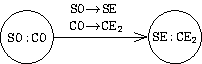
\includegraphics[scale=1.35]{chapters/figures/figIsEmptyProductCfg.pdf}
\end{center}
\vspace{6.5px}
\caption{\label{fig:isemptyproductcfg}Product-CFG between \cref{fig:isemptyspeccfg,fig:isemptyccfg}}
\end{subfigure}%
&
\begin{subfigure}[b]{0.55\textwidth}
\begin{center}
\begin{footnotesize}
\begin{tabular}{cl}
\toprule
{\bf PC-Pair} & \multicolumn{1}{c}{\bf Invariants} \\
\toprule
(\scpc{0}{0}) & $\circled{P}\  \sv{s} \indEq{} \lifted{str}{\mem{}}{u8[]}{\cv{s}}$ \\
\midrule
(\scpc{E}{E_2}) & $\circled{E} \  \sv{ret} = \cv{ret}$ \\
\bottomrule
\end{tabular}
\end{footnotesize}
\end{center}
\caption{\label{fig:isemptyinvs}Invariants table for product-CFG in \cref{fig:isemptyproductcfg}}
\end{subfigure}%
\\
\end{tabular}
\caption{\label{fig:isemptyproductcfgandinvs}Product-CFG and its associated node invariants for CFGs in \cref{fig:isemptyspeccfg,fig:isemptyccfg}.}
\end{figure}


Since \SpecL{} has no notion of pointers, we expose this conditional well-formedness of C input \cv{s}
through an explicit data constructor \cons{SInvalid} for the \type{Str} ADT defined in \apc{0} in \cref{fig:isemptyspec}.
Additionally, \sdef{} asserts $\neg(\sumIs{\sv{s}}{SInvalid})$ (in \apc{4} and \spath{1,2} in \cref{fig:isemptyspecir}) and the precondition \pre{}
(labeled \circled{P} in \cref{fig:isemptyinvs}) relates $(\sumIs{\sv{s}}{SInvalid}) \Leftrightarrow (\cv{s} = 0_\type{i32})$\footnote{
The relation is implied by the \recursiveRelation{} $\sv{l} \indEq{} \lifted{str}{\mem{}}{u8[]}{\cv{l}}$ as part of \pre{} shown in \cref{fig:isemptyinvs}.
The lifting constructor $\lift{str}{\mem{}}{u8[]}$ is defined subsequently in \cref{sec:recrel}.}.
Combined, \sdef{} and \pre{} ensure that we constrain the inputs of \sprog{} and in turn, \cprog{} to only well-formed values
during equivalence check.
A similar strategy is employed for functions from the standard library (e.g. {\tt strchr}) and is explored in detail
during evaluation in \cref{sec:strchrexample}.

\begin{figure}
\begin{tabular}{cc}
\begin{subfigure}[b]{0.45\textwidth}
\begin{center}
{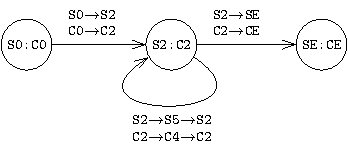
\includegraphics[scale=1.1]{chapters/figures/figSumListProductCfg.pdf}}
\end{center}
\caption{\label{fig:llTraverseProduct}Product-CFG}
\end{subfigure}%
&
\begin{subfigure}[b]{0.55\textwidth}
\begin{center}
\begin{footnotesize}
\begin{tabular}{|c|l|}
\hline
{\bf PC-Pair} & \multicolumn{1}{c|} {\bf Invariants} \\
\hline
\hline
(\scpc{0}{0}) &
\Tstrut $\circled{P}\  \sv{l} \indEq{} \lifted{list}{\mem{}}{lnode}{\cv{l}}$ \\
\multirow{2}{*}{(\scpc{2}{2})} &
\Tstrut $\circled{\scriptsize I1}\  \sv{l} \indEq{} \lifted{list}{\mem{}}{lnode}{\cv{l}}$ \\ &
\Tstrut $\circled{\scriptsize I2}\  \sv{sum} = \cv{sum}$ \\
(\scpc{E}{E}) &
\Tstrut $\circled{\scriptsize E}\  \sv{ret} = \cv{ret}$ \\
\hline
\end{tabular}
\end{footnotesize}
\vspace{13px}
\end{center}
\caption{\label{fig:llTraverseProductInv}Node Invariants of the Product-CFG}
\end{subfigure}%
\\
\end{tabular}
\caption{\label{fig:llTraverseProductCFGInvs} Product-CFG between the IRs in \cref{fig:llTraverseSpec,fig:llTraverseC}. The inductive invariants of the Product-CFG are given in \cref{fig:llTraverseProductInv}.}
\end{figure}


\section{Bisimulation Relation}
\label{sec:bisim}
Recall that,
we construct a {\em bisimulation relation} to identify equivalence between the CFGs of \SpecL{} and C procedures.
A bisimulation relation correlates the transitions of \sprog{} and \cprog{} in lockstep, such that the
lockstep execution ensures identical observable behaviour.
A bisimulation relation between two programs can be represented using a {\em product program}
\cite{covac} and the CFG representation of a product program is called a {\em product}-CFG.
\Cref{fig:llTraverseProduct} shows a product-CFG, that encodes the lockstep execution
(bisimulation relation) between the CFGs in \cref{fig:llTraverseSpecCFG,fig:llTraverseCCFG}.

A node in the product-CFG is formed by pairing nodes of \sprog{} and \cprog{},
e.g., (\scpc{2}{2}) is formed by pairing \spc{2} and \cpc{2}.
If the lockstep execution of both programs is at node (\scpc{2}{2}) in the product-CFG,
then \sprog{}'s execution is at \spc{2} and \cprog{}'s execution is at \cpc{2}.
The start node (\scpc{0}{0}) of the product-CFG correlates the start nodes of CFGs of \sprog{} and \cprog{}.
Similarly, the exit node (\scpc{E}{E}) correlates the exit nodes of both programs.

An edge in the product-CFG is formed by pairing a {\em path} (a sequence of edges) in \sprog{}
with a path in \cprog{}\footnote{
For ease of exposition, we present product-CFG in the context of {\em path} correlations.
However, a more general approach of pathset is used based on prior work \cite{oopsla20}
for improved completeness of our algorithm.
We will explore pathsets and its consequences on the algorithm in more detail in \cref{sec:pathsetcorrel}.}.
A product-CFG edge encodes the lockstep execution of its correlated paths.
For example, the product-CFG edge \scedge{2}{2}{2}{2} is formed by pairing
\spath{2,5,2} and \cpath{2,4,2} in \cref{fig:llTraverseSpecCFG,fig:llTraverseCCFG} respectively,
and represents that when \sprog{} makes the transition \spath{2,5,2}, \cprog{} makes the transition \cpath{2,4,2}
in lockstep.
In general, a product-CFG edge $e$ may correlate a finite path \sv{\rho} in \sprog{} with a finite path
\cv{\rho} in \cprog{}, written $e=(\sv{\rho},\cv{\rho})$.
The empty path $\epsilon$ in \sprog{} may be correlated with a finite path in \cprog{},
effectively simulating a {\em stuttering bisimulation} relation.

At the start node (\scpc{0}{0}) of the product-CFG in \cref{fig:llTraverseProduct},
the precondition \pre{} (labeled \circled{\small P})
ensures equality of input lists \sv{l} and \cv{l} at procedure entries.
{\em Inductive invariants} (labeled \circled{I}) are inferred
at each intermediate product-CFG node (e.g., (\scpc{2}{2})) that relate
the values of \sprog{} with values and memory state of \cprog{}.
At the exit node (\scpc{E}{E}) of the product-CFG, the postcondition \post{} (labeled \circled{\small E})
represents equality of observable outputs and forms our overall proof obligation.
Assuming that the precondition \pre{} (\circled{\small P}) holds at the entry node (\scpc{0}{0}),
a bisimulation check involves checking that the inductive invariants (\circled{\small I}) hold too,
and consequently the postcondition \post{} (\circled{\small E}) holds at the exit node (\scpc{E}{E}).
The input-output specification (i.e. $(\pre{},\post{})$) is manually provided by the user
while all inductive invariants are identified by an invariant inference algorithm described in \cref{sec:invinferalgo}.

\subsection{Well-formedness of Product-CFG}
A product-CFG is well-formed (i.e. represents a valid bisimulation relation) if it correlates every {\em possibly} executable
edge (as part of a path) in \cprog{} with a path in \sprog{}.
An edge deemed to be unreachable (due to an unsatisfiable path condition) represents {\em dead code} and can be
safely ignored and remain uncorrelated in the final product-CFG.
For example, the \sdef{} and \pre{} conditions assert unreachability of the edge \cpath{0,E_1} in \cref{fig:isemptyccfg},
and remain uncorrelated in the product-CFG in \cref{fig:isemptyproductcfg}.
Without \sdef{} and \pre{}, our equivalence checker would fail because the edge \cpath{0,E_1} is only triggered for ill-formed
inputs and has no correlated paths in its specification.

Additionally, a well-formed product-CFG may not correlate a loop path in \cprog{} with the empty path $\epsilon$ in \sprog{}.
For example, \cref{fig:llAllocProductCFG} shows the product-CFG between the programs
in \cref{fig:llAllocSpecIRCFG,fig:llAllocCCFG} respectively.
The edges \scedge{3}{3}{3}{4} and \scedge{3}{4}{3}{5} correlate the empty path $\epsilon$
with the non-empty paths \cpath{3,4} and \cpath{4,5} respectively.
However, the only loop path \cpath{3,4,5,3} in \cprog{} is still correlated with the non-empty path \spath{3,5,3}
in \sprog{} and thus, the product-CFG in \cref{fig:llAllocProductCFG} satisfies this well-formedness criterion.
This well-formedness condition ensures {\em divergence}, i.e. either both programs terminate or
both continue indefinitely.

\section{Recursive Relation}
\label{sec:recrel}
In \cref{sec:motivatingexample}, we briefly introduced a lifting constructor (\lift{list}{\mem{}}{lnode})
and associated \recursiveRelations{}.
In \cref{fig:llTraverseProductInv}, the precondition (\circled{\small P}) is another instance
of a \recursiveRelation{}:
``\sv{l} \indEq{} \lifted{list}{\mem{}}{lnode}{\cv{l}}'' where \sv{l} and \cv{l}
represent the input arguments to the \SpecL{} and C procedures respectively,
\type{lnode} is the C \type{struct} type that contains the \field{val} and \field{next} fields (defined at \bpc{0} in \cref{fig:llTraverseC}),
and \mem{} is the byte-addressable array representing the current memory state of the C program.
$l_1 \indEq{} l_2$ is read {\em $l_1$ is recursively equal to $l_2$} and is semantically equivalent
to $l_1 = l_2$. The `\indEq{}' simply emphasizes that $l_1$ and $l_2$ are (possibly recursive) ADT values.
The lifting constructor \lift{list}{\mem{}}{lnode} `lifts' a C pointer value $p$
(pointing to an object of type \type{struct lnode}) and
memory state \mem{} to a (possibly infinite in case of a circular list) \type{List} value,
and is defined through its {\em unrolling procedure} as follows:

\begin{equation}
\label{eqn:clist}
\begin{aligned}
U_C:\ \lifted{list}{\mem{}}{lnode}{p \ctype{i32}} = \ & \sumIf{p=0} \ \sumThen{\cons{LNil}} \\
                                                      & \sumElse{\cons{LCons}(\structPointer{p}{\mem{}}{lnode}{val}, \lifted{list}{\mem{}}{lnode}{\structPointer{p}{\mem{}}{lnode}{next}})}
\end{aligned}
\end{equation}

Note the recursive nature of the lifting constructor \lift{list}{\mem{}}{lnode}: if the pointer $p$ is zero
(i.e. $p$ is a null pointer), then it represents the empty list \cons{LNil};
otherwise it represents the list formed by \cons{LCons}-ing the value stored at
\structPointer{p}{\mem{}}{lnode}{val} in memory \mem{} and the list formed by recursively
lifting \structPointer{p}{\mem{}}{lnode}{next} through \lift{list}{\mem{}}{lnode}.
\lifted{list}{\mem{}}{lnode}{p} allows us to adapt a C linked list (formed by chasing pointers
in the memory \mem{}) to a \type{List} value and compare it with a \SpecL{} \type{List}
value for equality.

Also, consider the \type{Str} lifting constructor \lift{str}{\mem{}}{u8[]} (in \cref{fig:isemptyinvs}) used to lift a null-character
terminated C string into a \type{Str} value.
Similar to the \type{List} lifting constructor, \lift{str}{\mem{}}{u8[]} is also defined through its unrolling procedure as follows:

\begin{equation}
\label{eqn:cstr}
\begin{aligned}
\lifted{str}{\mem{}}{u8[]}{p \ctype{i32}} = \ & \sumIf{p=0} \ \sumThen{\cons{SInvalid}} \\
                                              & \sumElif{\arrIndex{p}{0}{\mem{}}{i8} = 0} \ \sumThen{\cons{SNil}} \\
                                              & \sumElse{\cons{SCons}(\arrIndex{p}{0}{\mem{}}{i8}, \lifted{str}{\mem{}}{u8[]}{p+1})}
\end{aligned}
\end{equation}

Observe that an ill-formed string is related to the pointer being null,
while a null character represents the empty string.

\section{Proof Obligations}
\label{sec:proofobl}
As previously discussed, algorithms for (a) incremental construction of a Product-CFG
and (b) inference of invariants at intermediate PCs in the (partially constructed) product-CFG, are
based on prior work\cite{oopsla20} and discussed subsequently in \cref{sec:searchalgo,sec:invinferalgo}.
We discuss the proof obligations that arise from a given product-CFG.
Recall that a bisimulation check involves checking that all inductive invariants
(and the postcondition \post{}) hold at their associated product-CFG nodes.
Additionally, if a product-CFG correlates paths $\sv{\rho}$ and $\cv{\rho}$ (in \sprog{} and \cprog{}),
a bisimulation check must ensure that their respective path conditions are {\em compatible}\footnote{
Paths $\sv{\rho}$ and $\cv{\rho}$ are {\em compatible} if whenever \cprog{} executes $\cv{\rho}$,
\sprog{} executes $\sv{\rho}$, i.e. ${\tt pathcond}_{\cv{\rho}} \Rightarrow {\tt pathcond}_{\sv{\rho}}$.}
(under the appropriate node invariants).

We use relational Hoare triples to express these proof obligations \cite{relationalHoareLogic,hoareTriple}.
If $\phi$ denotes a predicate relating the machine states of \sprog{} and \cprog{}, then
for a product-CFG edge $e=(\sv{\rho},\cv{\rho})$, \hoareTriple{\phi_s}{e}{\phi_d}
denotes the condition:
if any machine states \sv{\sigma} and \cv{\sigma} of programs \sprog{} and \cprog{} are related through
precondition $\phi_s(\sv{\sigma},\cv{\sigma})$ and the finite paths \sv{\rho} and \cv{\rho}
are executed in \sprog{} and \cprog{} respectively,
then execution terminates normally in states $\sv{\sigma}^{'}$ (for \sprog{}) and
$\cv{\sigma}^{'}$ (for \cprog{}) and postcondition $\phi_d(\sv{\sigma}^{'},\cv{\sigma}^{'})$ holds.

For every product-CFG edge $e = (s \rightarrow d) = (\sv{\rho}, \cv{\rho})$,
we are interested in proving: \hoareTriple{\phi_s}{\sv{\rho},\cv{\rho}}{\phi_d},
where $\phi_s$ and $\phi_d$ are the node invariants at the product-CFG nodes $s$ and $d$
respectively.
The weakest-precondition transformer is used to translate a Hoare triple
\hoareTriple{\phi_s}{\sv{\rho},\cv{\rho}}{\phi_d} to the following
first-order logic formula:

\begin{equation}
\label{eqn:firstOrderFormula}
(\phi_s \land {\tt pathcond}_{\sv{\rho}} \land {\tt pathcond}_{\cv{\rho}} \land {\tt ubfree}_{\sv{\rho}}) \Rightarrow {\tt WP}_{{\sv{\rho},\cv{\rho}}}(\phi_d)
\end{equation}

Here, ${\tt pathcond}_{\rho_X}$ represents the condition that path $\rho$ is taken in program $X$
and ${\tt ubfree}_{\sv{\rho}}$ represents the condition that execution of \sprog{} along path $\sv{\rho}$
is free of undefined behaviour.
${\tt WP}_{{\sv{\rho},\cv{\rho}}}(\phi_d)$ represents the weakest-precondition
of the predicate $\phi_d$ across the product-CFG edge $e = (\sv{\rho},\cv{\rho})$.
From now on, we will use `\lhs{}' and `\rhs{}' to refer to the antecedent and consequent of
the implication operator `$\Rightarrow$' in \cref{eqn:firstOrderFormula}.

For example, checking that the loop invariant \circled{\small I2}
$\sv{l} \indEq{} \lifted{list}{\mem{}}{lnode}{\cv{l}}$ holds at (\scpc{2}{2}) in \cref{fig:llTraverseProduct}
requires us to prove the following two proof obligations:
\circled{1} \hoareTriple{\scpcinv{0}{0}}{\spath{0,2},\cpath{0,2}}{\sv{l} \indEq{} \lifted{list}{\mem{}}{lnode}{\cv{l}}} and
\circled{2} \hoareTriple{\scpcinv{2}{2}}{\spath{2,5,2},\cpath{2,4,2}}{\sv{l} \indEq{} \lifted{list}{\mem{}}{lnode}{\cv{l}}}.
Using weakest precondition predicate transformer, the proof obligation \circled{2} reduces to the following first-order logic formula:

\begin{equation}
\label{eqn:firstOrderFormulaExample}
\begin{aligned}
\sv{l} \indEq{} \lifted{list}{\mem{}}{lnode}{\cv{l}} &\land \sv{sum} = \cv{sum} \land (\sumIs{\sv{l}}{LCons}) \land (\cv{l} \neq 0) \\
&\Rightarrow \prodAccess{\sv{l}}{next} \indEq{} \lifted{list}{\mem{}}{lnode}{\structPointer{\cv{l}}{\mem{}}{lnode}{next}}
\end{aligned}
\end{equation}

Due to the presence of \recursiveRelations{}, these proof queries
(e.g., \cref{eqn:firstOrderFormulaExample}) cannot be solved directly by
off-the-shelf solvers and require special handling.
The next chapter illustrates our proof discharge algorithm for solving proof queries
involving \recursiveRelations{}.
